\chapter{Introduction}
\label{ch:introduction}


\newpage

\section{Introduction}

%\begin{itemize}
%
%    \item What is the subject of the study? Describe the
%        economic/econometric problem.
%
%    \item What is the purpose of the study (working hypothesis)?
%
%    \item What do we already know about the subject (literature
%        review)? Use citations: {\it \citet{Gallant:87} shows that...
%        Alternative Forms of the Wald test are considered
%        \citep{Breusch&Schmidt:88}.}
%
%    \item What is the innovation of the study?
%
%    \item Provide an overview of your results.
%
%
%    \item Outline of the paper:\\
%        {\it The paper is organized as follows. The next section describes %the
%        model under investigation. Section \ref{Sec:Literature Review} %reviews the up-to-date research works.
%        and Section \ref{Sec:Results} presents the results. Finally, %Section
%        \ref{Sec:Conc} concludes.}
%
%    \item The introduction should not be longer than 4 pages.
%
%\end{itemize}




\par More and more the usage of RDF is increasing in many fields in computer science. RDF data representation helps in supporting the machine to perform the normally manual computation work in an automatic fashion. Moreover, the machines will be smarter to understand the data which is represented in RDF format. 
\vspace{5mm} %5mm vertical space


The quality of RDF data needs to be ensure before proceeding of any further processing. Most of current parsers which focus on detection of the syntax error fail to detect more than one error, especially, of RDF data represented in Turtle or NTriples format. 

\vspace{5mm} %5mm vertical space

This study was encouraged by the tremendous data representation of either Turtle and NTriples. Hence, the intention of the study to afford a user-friendly syntax checker or parser. Such parser or syntax checker should give all errors can be detect inside such data.


			



\subsection{Motivation}

This study was motivated by several scenarios which require syntax checking of RDF data as an input and ensuring of its quality. To mention one of such scenarios, let's discuss an example shown in {\it Figure \ref{Fig:Motivation}. The example describes a collaboration system for processing an input data, say for example to perform machine learning analysis. Of course,in a such case, a valid input data to the system is must. The input data is verified for further data processing. Most of the current existing systems  ensuring syntax-error-free RDF data, are stopped parsing at the first syntax error occurrence, as will be followed in Section \ref{Sec:Review}.
	\vspace{5mm} %5mm vertical space
	\par
	To stop parsing when the first syntax error is found will introduce much complications. Assuming, the input RDF data contains, for example, 10 syntax errors. Normally, what is happing when an error is found, the system will proceed with no further processing, instead it will report error's existence in the inserted data. The reported error then should be corrected by the user, then after correction data will be send back for re-checking of data's syntax. To make it more complex, imagine that the user will do such correction process for 10 times (remember that data includes 10 errors). Then, what if the data contains hundreds or thousands of errors. 

	\begin{figure}[ht]
		\begin{center}
			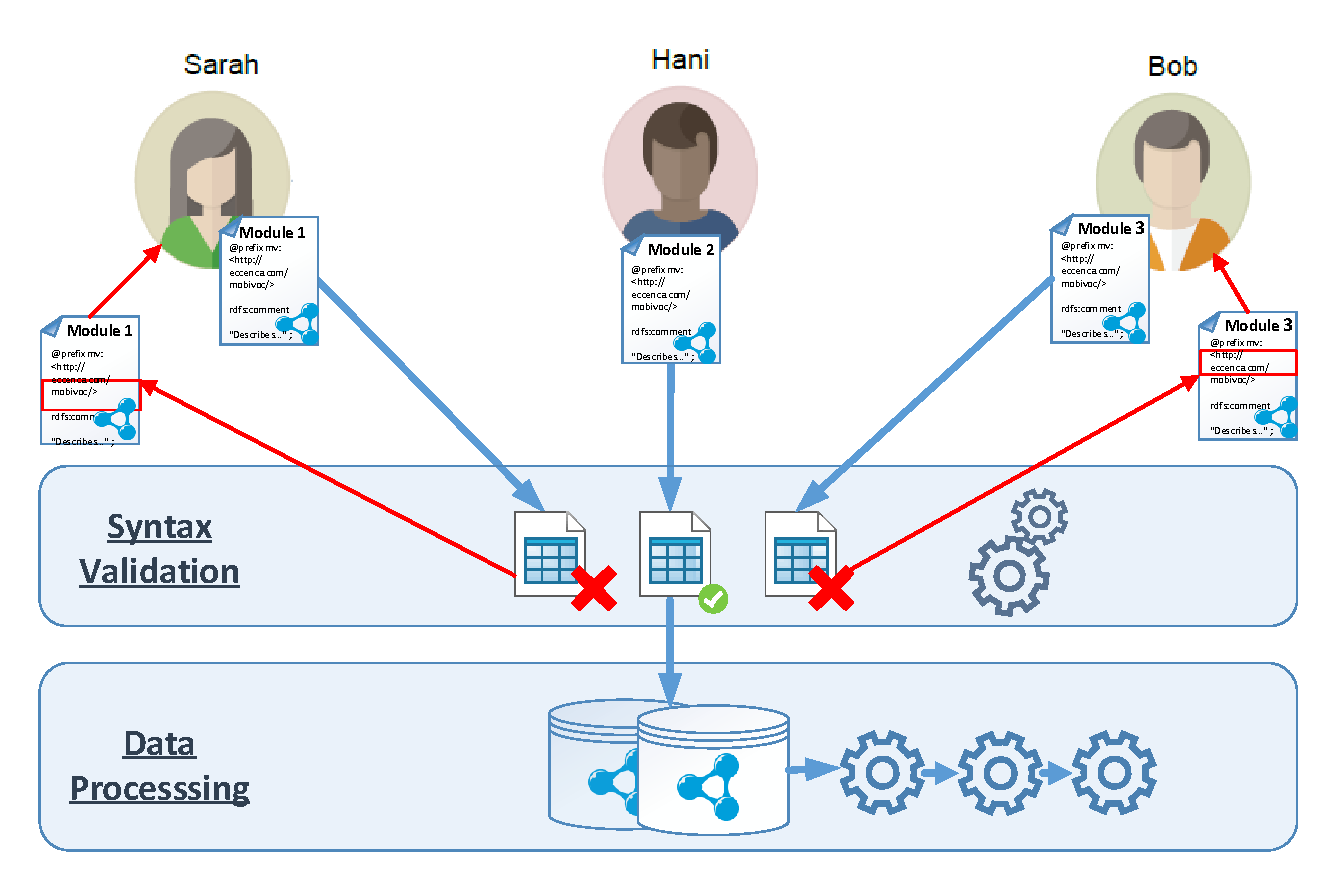
\includegraphics[scale=0.5,angle=0]{images/motivation}
			\caption{A motivation example of syntax checking of data before further processing}
			\label{Fig:Motivation}
		\end{center}
	\end{figure}
	\vspace{8mm} %5mm vertical space
	
	let's dig deep to explain what is there in  {\it Figure \ref{Fig:Motivation}, It is showing a flow of data from clients or users seeking further data processing. 3 persons are shown in this Figure, their names are Bob, Hani, and Sarah. All of them start with the first phase by sending the data to be syntacticly checked. The parser starts checking if there syntax errors of the input data, then if such data passed with no syntax errors, it can be forwarded for further phases, i.e. for data processing, otherwise, the input data will send back to the user to correct the errors. {\it Figure \ref{Fig:Motivation} clearly shows that Sarah and Bob have syntax errors in their input data,then they got an error report, including found errors. In the meanwhile, Hani has received his data processed without getting such an error report, since his input data has no syntax errors. 
			\vspace{5mm} %5mm vertical space
			\par
			This study has been encouraged by the illustrated example to find a suitable solution for such cases. The proposed solution will focus on producing a software program that can detect all or almost syntax errors that can be detected in the input data. 

%\section{Objectives}
\section{Proposed Problem } 	
The tackled problem in this study is to list all the detected syntax errors found in RDF files; in order to help ontology engineers and users to fix them in one shut. Such a list of errors provided in the output of the syntax checking phase will significantly assist to get rid of a loop of first error notification if multiple errors are found in the input data.  

\section {Contributions}

			The contributions of this study are:
\begin{enumerate}

	\item  {\bf Reporting list of detected syntax errors found in RDF data:} 
	\item {\bf  Showing expressive error messages: }
	\item {\bf Correcting some errors: }
	
	
	
	
	

\end{enumerate}


\section {Thesis Structure}

The remainder of this document is structured as follows. In the \nameref{ch:related} chapter

			The thesis is organized as follows. The next section presents the
problem description. Section \ref{Sec:Review} reviews the up-to-date research works. Section \ref{Sec:Data} describes the data set
and Section \ref{Sec:Results} presents the results. Finally, Section
\ref{Sec:Conc} concludes





